\documentclass[twoside]{book}

% Packages required by doxygen
\usepackage{fixltx2e}
\usepackage{calc}
\usepackage{doxygen}
\usepackage[export]{adjustbox} % also loads graphicx
\usepackage{graphicx}
\usepackage[utf8]{inputenc}
\usepackage{makeidx}
\usepackage{multicol}
\usepackage{multirow}
\PassOptionsToPackage{warn}{textcomp}
\usepackage{textcomp}
\usepackage[nointegrals]{wasysym}
\usepackage[table]{xcolor}

% Font selection
\usepackage[T1]{fontenc}
\usepackage[scaled=.90]{helvet}
\usepackage{courier}
\usepackage{amssymb}
\usepackage{sectsty}
\renewcommand{\familydefault}{\sfdefault}
\allsectionsfont{%
  \fontseries{bc}\selectfont%
  \color{darkgray}%
}
\renewcommand{\DoxyLabelFont}{%
  \fontseries{bc}\selectfont%
  \color{darkgray}%
}
\newcommand{\+}{\discretionary{\mbox{\scriptsize$\hookleftarrow$}}{}{}}

% Page & text layout
\usepackage{geometry}
\geometry{%
  a4paper,%
  top=2.5cm,%
  bottom=2.5cm,%
  left=2.5cm,%
  right=2.5cm%
}
\tolerance=750
\hfuzz=15pt
\hbadness=750
\setlength{\emergencystretch}{15pt}
\setlength{\parindent}{0cm}
\setlength{\parskip}{3ex plus 2ex minus 2ex}
\makeatletter
\renewcommand{\paragraph}{%
  \@startsection{paragraph}{4}{0ex}{-1.0ex}{1.0ex}{%
    \normalfont\normalsize\bfseries\SS@parafont%
  }%
}
\renewcommand{\subparagraph}{%
  \@startsection{subparagraph}{5}{0ex}{-1.0ex}{1.0ex}{%
    \normalfont\normalsize\bfseries\SS@subparafont%
  }%
}
\makeatother

% Headers & footers
\usepackage{fancyhdr}
\pagestyle{fancyplain}
\fancyhead[LE]{\fancyplain{}{\bfseries\thepage}}
\fancyhead[CE]{\fancyplain{}{}}
\fancyhead[RE]{\fancyplain{}{\bfseries\leftmark}}
\fancyhead[LO]{\fancyplain{}{\bfseries\rightmark}}
\fancyhead[CO]{\fancyplain{}{}}
\fancyhead[RO]{\fancyplain{}{\bfseries\thepage}}
\fancyfoot[LE]{\fancyplain{}{}}
\fancyfoot[CE]{\fancyplain{}{}}
\fancyfoot[RE]{\fancyplain{}{\bfseries\scriptsize Generated by Doxygen }}
\fancyfoot[LO]{\fancyplain{}{\bfseries\scriptsize Generated by Doxygen }}
\fancyfoot[CO]{\fancyplain{}{}}
\fancyfoot[RO]{\fancyplain{}{}}
\renewcommand{\footrulewidth}{0.4pt}
\renewcommand{\chaptermark}[1]{%
  \markboth{#1}{}%
}
\renewcommand{\sectionmark}[1]{%
  \markright{\thesection\ #1}%
}

% Indices & bibliography
\usepackage{natbib}
\usepackage[titles]{tocloft}
\setcounter{tocdepth}{3}
\setcounter{secnumdepth}{5}
\makeindex

% Hyperlinks (required, but should be loaded last)
\usepackage{ifpdf}
\ifpdf
  \usepackage[pdftex,pagebackref=true]{hyperref}
\else
  \usepackage[ps2pdf,pagebackref=true]{hyperref}
\fi
\hypersetup{%
  colorlinks=true,%
  linkcolor=blue,%
  citecolor=blue,%
  unicode%
}

% Custom commands
\newcommand{\clearemptydoublepage}{%
  \newpage{\pagestyle{empty}\cleardoublepage}%
}

\usepackage{caption}
\captionsetup{labelsep=space,justification=centering,font={bf},singlelinecheck=off,skip=4pt,position=top}

%===== C O N T E N T S =====

\begin{document}

% Titlepage & ToC
\hypersetup{pageanchor=false,
             bookmarksnumbered=true,
             pdfencoding=unicode
            }
\pagenumbering{alph}
\begin{titlepage}
\vspace*{7cm}
\begin{center}%
{\Large V\+D\+S\+Project \\[1ex]\large 1.\+0 }\\
\vspace*{1cm}
{\large Generated by Doxygen 1.8.13}\\
\end{center}
\end{titlepage}
\clearemptydoublepage
\pagenumbering{roman}
\tableofcontents
\clearemptydoublepage
\pagenumbering{arabic}
\hypersetup{pageanchor=true}

%--- Begin generated contents ---
\chapter{B\+DD package}
\label{index}\hypertarget{index}{}\hypertarget{index_intro_sec}{}\section{Introduction}\label{index_intro_sec}
A package for working with Ordered Binary Decision Diagrams (O\+B\+D\+Ds) is provided.

This package allows to reduce said data structures, obtaining equivalent R\+O\+B\+D\+Ds. In order to do so, the if-\/then-\/else (I\+TE) algorithm is used, together with the corresponding unique and computed tables.\hypertarget{index_used_sec}{}\section{Techniques and tools used}\label{index_used_sec}
This package has been implemented in C++ using C\+Lion as I\+DE. Also, this has been done using Test Driven Develpment (T\+DD), with the tests being implemented using Gtest. Finally, this documentation has been generated using Doxygen.\hypertarget{index_devs_sec}{}\section{Developers}\label{index_devs_sec}
This package has been developed by\+:
\begin{DoxyItemize}
\item Dino Mehmedagić
\item Juan Felipe Vargas Colorado
\item Mateo Vázquez Maceiras 
\end{DoxyItemize}
\chapter{Hierarchical Index}
\section{Class Hierarchy}
This inheritance list is sorted roughly, but not completely, alphabetically\+:\begin{DoxyCompactList}
\item \contentsline{section}{c\+Table\+Val}{\pageref{structcTableVal}}{}
\item \contentsline{section}{Manager\+Interface}{\pageref{classManagerInterface}}{}
\begin{DoxyCompactList}
\item \contentsline{section}{Manager}{\pageref{classManager}}{}
\end{DoxyCompactList}
\item \contentsline{section}{u\+Table\+Val}{\pageref{structuTableVal}}{}
\end{DoxyCompactList}

\chapter{Class Index}
\section{Class List}
Here are the classes, structs, unions and interfaces with brief descriptions\+:\begin{DoxyCompactList}
\item\contentsline{section}{\hyperlink{classClassProject_1_1Manager}{Class\+Project\+::\+Manager} \\*Implements the interface of the B\+DD package }{\pageref{classClassProject_1_1Manager}}{}
\item\contentsline{section}{\hyperlink{classClassProject_1_1ManagerInterface}{Class\+Project\+::\+Manager\+Interface} \\*Defines the implemented interface of the B\+DD package }{\pageref{classClassProject_1_1ManagerInterface}}{}
\item\contentsline{section}{\hyperlink{classClassProject_1_1Reachable}{Class\+Project\+::\+Reachable} \\*Implements the interface of the reachability extension }{\pageref{classClassProject_1_1Reachable}}{}
\item\contentsline{section}{\hyperlink{classClassProject_1_1ReachableInterface}{Class\+Project\+::\+Reachable\+Interface} \\*Defines the implemented interface of the reachability extension }{\pageref{classClassProject_1_1ReachableInterface}}{}
\item\contentsline{section}{\hyperlink{structClassProject_1_1uTableVal}{Class\+Project\+::u\+Table\+Val} \\*Struct used as value in the unique table }{\pageref{structClassProject_1_1uTableVal}}{}
\end{DoxyCompactList}

\chapter{Class Documentation}
\hypertarget{structcTableVal}{}\section{c\+Table\+Val Struct Reference}
\label{structcTableVal}\index{c\+Table\+Val@{c\+Table\+Val}}


Struct used as value in the computed table.  




{\ttfamily \#include $<$Manager.\+h$>$}

\subsection*{Public Member Functions}
\begin{DoxyCompactItemize}
\item 
\mbox{\Hypertarget{structcTableVal_a22fc4897c20dbe73c37a8e1923f9ca7c}\label{structcTableVal_a22fc4897c20dbe73c37a8e1923f9ca7c}} 
{\bfseries c\+Table\+Val} (B\+D\+D\+\_\+\+ID \+\_\+i, B\+D\+D\+\_\+\+ID \+\_\+t, B\+D\+D\+\_\+\+ID \+\_\+e)
\end{DoxyCompactItemize}
\subsection*{Public Attributes}
\begin{DoxyCompactItemize}
\item 
\mbox{\Hypertarget{structcTableVal_a3600ed12ce2bb26e93ce5c2e00a98d3a}\label{structcTableVal_a3600ed12ce2bb26e93ce5c2e00a98d3a}} 
B\+D\+D\+\_\+\+ID {\bfseries i}
\item 
\mbox{\Hypertarget{structcTableVal_a6310500b8caae666044f1a8aac20af3a}\label{structcTableVal_a6310500b8caae666044f1a8aac20af3a}} 
B\+D\+D\+\_\+\+ID {\bfseries t}
\item 
\mbox{\Hypertarget{structcTableVal_aa68a08fe21dd1acb23eb0ac3be8b5d15}\label{structcTableVal_aa68a08fe21dd1acb23eb0ac3be8b5d15}} 
B\+D\+D\+\_\+\+ID {\bfseries e}
\end{DoxyCompactItemize}


\subsection{Detailed Description}
Struct used as value in the computed table. 

This data structure contains the arguments of previously calculated i-\/t-\/e combinations 
\hypertarget{classManager}{}\section{Manager Class Reference}
\label{classManager}\index{Manager@{Manager}}


Inheritance diagram for Manager\+:
\nopagebreak
\begin{figure}[H]
\begin{center}
\leavevmode
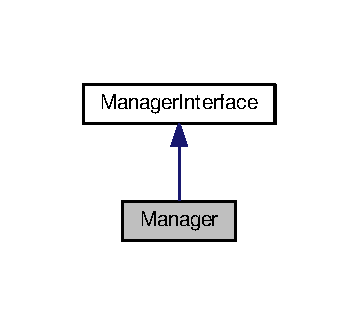
\includegraphics[width=172pt]{classManager__inherit__graph}
\end{center}
\end{figure}


Collaboration diagram for Manager\+:
\nopagebreak
\begin{figure}[H]
\begin{center}
\leavevmode
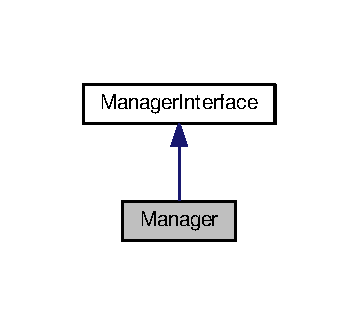
\includegraphics[width=172pt]{classManager__coll__graph}
\end{center}
\end{figure}
\subsection*{Public Member Functions}
\begin{DoxyCompactItemize}
\item 
\hyperlink{classManager_a1658ff9f18e38ccd9cb8b0b371b9c20b}{Manager} ()
\begin{DoxyCompactList}\small\item\em Constructor. \end{DoxyCompactList}\item 
const B\+D\+D\+\_\+\+ID \& \hyperlink{classManager_a0c15aff167a7019502b66100c4ec0a33}{True} ()
\item 
const B\+D\+D\+\_\+\+ID \& \hyperlink{classManager_ae9bae01509e6063313024cd85a8eb569}{False} ()
\item 
bool \hyperlink{classManager_a98fe06b67d8114f1404a7b19dddc935b}{is\+Constant} (const B\+D\+D\+\_\+\+ID f)
\item 
bool \hyperlink{classManager_af026f76f68823bb9083f161b5db9e58b}{is\+Variable} (const B\+D\+D\+\_\+\+ID x)
\item 
B\+D\+D\+\_\+\+ID \hyperlink{classManager_a9fb480d8af44c75ee2b35b85f7038e68}{create\+Var} (const std\+::string \&label)
\end{DoxyCompactItemize}


\subsection{Constructor \& Destructor Documentation}
\index{Manager@{Manager}!Manager@{Manager}}
\index{Manager@{Manager}!Manager@{Manager}}
\subsubsection[{\texorpdfstring{Manager()}{Manager()}}]{\setlength{\rightskip}{0pt plus 5cm}Manager\+::\+Manager (
\begin{DoxyParamCaption}
{}
\end{DoxyParamCaption}
)}\hypertarget{classManager_a1658ff9f18e38ccd9cb8b0b371b9c20b}{}\label{classManager_a1658ff9f18e38ccd9cb8b0b371b9c20b}


Constructor. 

This constructor creates the unique table to store the values of the R\+O\+B\+DD. It also adds the values of \textquotesingle{}0\textquotesingle{} and \textquotesingle{}1\textquotesingle{} to the table, where the ID of \textquotesingle{}0\textquotesingle{} corresponds to 0 and the ID of \textquotesingle{}1\textquotesingle{} is 1 

\subsection{Member Function Documentation}
\index{Manager@{Manager}!create\+Var@{create\+Var}}
\index{create\+Var@{create\+Var}!Manager@{Manager}}
\subsubsection[{\texorpdfstring{create\+Var(const std\+::string \&label)}{createVar(const std::string &label)}}]{\setlength{\rightskip}{0pt plus 5cm}B\+D\+D\+\_\+\+ID Manager\+::create\+Var (
\begin{DoxyParamCaption}
\item[{const std\+::string \&}]{label}
\end{DoxyParamCaption}
)\hspace{0.3cm}{\ttfamily [virtual]}}\hypertarget{classManager_a9fb480d8af44c75ee2b35b85f7038e68}{}\label{classManager_a9fb480d8af44c75ee2b35b85f7038e68}
Creates a new variable for the B\+DD. 

Implements \hyperlink{classManagerInterface}{Manager\+Interface}.

\index{Manager@{Manager}!False@{False}}
\index{False@{False}!Manager@{Manager}}
\subsubsection[{\texorpdfstring{False()}{False()}}]{\setlength{\rightskip}{0pt plus 5cm}const B\+D\+D\+\_\+\+ID \& Manager\+::\+False (
\begin{DoxyParamCaption}
{}
\end{DoxyParamCaption}
)\hspace{0.3cm}{\ttfamily [virtual]}}\hypertarget{classManager_ae9bae01509e6063313024cd85a8eb569}{}\label{classManager_ae9bae01509e6063313024cd85a8eb569}
\begin{DoxyReturn}{Returns}
the ID of the node representing False. 
\end{DoxyReturn}


Implements \hyperlink{classManagerInterface}{Manager\+Interface}.

\index{Manager@{Manager}!is\+Constant@{is\+Constant}}
\index{is\+Constant@{is\+Constant}!Manager@{Manager}}
\subsubsection[{\texorpdfstring{is\+Constant(const B\+D\+D\+\_\+\+I\+D f)}{isConstant(const BDD_ID f)}}]{\setlength{\rightskip}{0pt plus 5cm}bool Manager\+::is\+Constant (
\begin{DoxyParamCaption}
\item[{const B\+D\+D\+\_\+\+ID}]{f}
\end{DoxyParamCaption}
)\hspace{0.3cm}{\ttfamily [virtual]}}\hypertarget{classManager_a98fe06b67d8114f1404a7b19dddc935b}{}\label{classManager_a98fe06b67d8114f1404a7b19dddc935b}
\begin{DoxyReturn}{Returns}
true if x is a leaf node. 
\end{DoxyReturn}


Implements \hyperlink{classManagerInterface}{Manager\+Interface}.

\index{Manager@{Manager}!is\+Variable@{is\+Variable}}
\index{is\+Variable@{is\+Variable}!Manager@{Manager}}
\subsubsection[{\texorpdfstring{is\+Variable(const B\+D\+D\+\_\+\+I\+D x)}{isVariable(const BDD_ID x)}}]{\setlength{\rightskip}{0pt plus 5cm}bool Manager\+::is\+Variable (
\begin{DoxyParamCaption}
\item[{const B\+D\+D\+\_\+\+ID}]{x}
\end{DoxyParamCaption}
)\hspace{0.3cm}{\ttfamily [virtual]}}\hypertarget{classManager_af026f76f68823bb9083f161b5db9e58b}{}\label{classManager_af026f76f68823bb9083f161b5db9e58b}
\begin{DoxyReturn}{Returns}
true if x is a variable. 
\end{DoxyReturn}


Implements \hyperlink{classManagerInterface}{Manager\+Interface}.

\index{Manager@{Manager}!True@{True}}
\index{True@{True}!Manager@{Manager}}
\subsubsection[{\texorpdfstring{True()}{True()}}]{\setlength{\rightskip}{0pt plus 5cm}const B\+D\+D\+\_\+\+ID \& Manager\+::\+True (
\begin{DoxyParamCaption}
{}
\end{DoxyParamCaption}
)\hspace{0.3cm}{\ttfamily [virtual]}}\hypertarget{classManager_a0c15aff167a7019502b66100c4ec0a33}{}\label{classManager_a0c15aff167a7019502b66100c4ec0a33}
\begin{DoxyReturn}{Returns}
the ID of the node representing True. 
\end{DoxyReturn}


Implements \hyperlink{classManagerInterface}{Manager\+Interface}.



The documentation for this class was generated from the following files\+:\begin{DoxyCompactItemize}
\item 
/home/juanvar/\+T\+U\+K/\+V\+D\+S/project/git/vdscp\+\_\+04/\+V\+D\+S\+Project/src/Manager.\+h\item 
/home/juanvar/\+T\+U\+K/\+V\+D\+S/project/git/vdscp\+\_\+04/\+V\+D\+S\+Project/src/Manager.\+cpp\end{DoxyCompactItemize}

\hypertarget{classManagerInterface}{}\section{Manager\+Interface Class Reference}
\label{classManagerInterface}\index{Manager\+Interface@{Manager\+Interface}}


Defines the implemented interface.  




{\ttfamily \#include $<$Manager\+Interface.\+h$>$}



Inheritance diagram for Manager\+Interface\+:\nopagebreak
\begin{figure}[H]
\begin{center}
\leavevmode
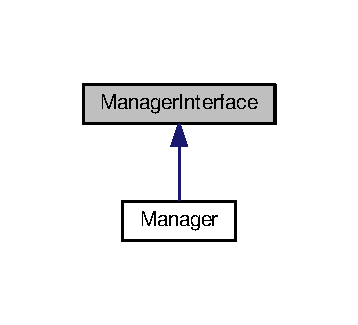
\includegraphics[width=172pt]{classManagerInterface__inherit__graph}
\end{center}
\end{figure}
\subsection*{Public Member Functions}
\begin{DoxyCompactItemize}
\item 
\mbox{\Hypertarget{classManagerInterface_a9c0561998e278c6f55dc9e1501786f73}\label{classManagerInterface_a9c0561998e278c6f55dc9e1501786f73}} 
\hyperlink{classManagerInterface_a9c0561998e278c6f55dc9e1501786f73}{Manager\+Interface} ()
\begin{DoxyCompactList}\small\item\em Constructor. \end{DoxyCompactList}\item 
virtual const B\+D\+D\+\_\+\+ID \& \hyperlink{classManagerInterface_abb06c4fac2f82fd9fc920afb395e7530}{True} ()=0
\item 
virtual const B\+D\+D\+\_\+\+ID \& \hyperlink{classManagerInterface_a8c5b3c1ebadc5c76e40e1648f5d459ca}{False} ()=0
\item 
virtual bool \hyperlink{classManagerInterface_a44d4002c509fa7a1c82747113ca0a09a}{is\+Constant} (const B\+D\+D\+\_\+\+ID f)=0
\item 
virtual bool \hyperlink{classManagerInterface_abed179c55a9e627784993ccfafca0841}{is\+Variable} (const B\+D\+D\+\_\+\+ID x)=0
\item 
virtual B\+D\+D\+\_\+\+ID \hyperlink{classManagerInterface_a89c9fcb50dcce71b530ead67c60b670f}{top\+Var} (const B\+D\+D\+\_\+\+ID f)=0
\item 
virtual B\+D\+D\+\_\+\+ID \hyperlink{classManagerInterface_a594a44f1304270f150257cfd5f7aa103}{create\+Var} (const std\+::string \&label)=0
\item 
virtual B\+D\+D\+\_\+\+ID \hyperlink{classManagerInterface_a099c8fab45923f6a30e4f2c53052e511}{ite} (const B\+D\+D\+\_\+\+ID i, const B\+D\+D\+\_\+\+ID t, const B\+D\+D\+\_\+\+ID e)=0
\item 
virtual B\+D\+D\+\_\+\+ID \hyperlink{classManagerInterface_a59efaa2b648ea1aa71da4bf0c817ee8c}{co\+Factor\+True} (const B\+D\+D\+\_\+\+ID f, B\+D\+D\+\_\+\+ID x)=0
\item 
virtual B\+D\+D\+\_\+\+ID \hyperlink{classManagerInterface_af5ea9287d7b926763f4972457ba067c7}{co\+Factor\+False} (const B\+D\+D\+\_\+\+ID f, B\+D\+D\+\_\+\+ID x)=0
\item 
virtual B\+D\+D\+\_\+\+ID \hyperlink{classManagerInterface_a205c88e6546302e6d41d4239b38ecb12}{co\+Factor\+True} (const B\+D\+D\+\_\+\+ID f)=0
\item 
virtual B\+D\+D\+\_\+\+ID \hyperlink{classManagerInterface_a8e4b1e439b4ce7d510d19ec1f45b03cf}{co\+Factor\+False} (const B\+D\+D\+\_\+\+ID f)=0
\item 
virtual B\+D\+D\+\_\+\+ID \hyperlink{classManagerInterface_ad3b2efbb8b99438198ab56c1a580e697}{and2} (const B\+D\+D\+\_\+\+ID a, const B\+D\+D\+\_\+\+ID b)=0
\item 
virtual B\+D\+D\+\_\+\+ID \hyperlink{classManagerInterface_abb14ac782d5527eb5dad1c1a456f6c5e}{or2} (const B\+D\+D\+\_\+\+ID a, const B\+D\+D\+\_\+\+ID b)=0
\item 
virtual B\+D\+D\+\_\+\+ID \hyperlink{classManagerInterface_a47d905e239650c255330b841edabd59d}{xor2} (const B\+D\+D\+\_\+\+ID a, const B\+D\+D\+\_\+\+ID b)=0
\item 
virtual B\+D\+D\+\_\+\+ID \hyperlink{classManagerInterface_af7c4261f0ae260de651909790d505555}{neg} (const B\+D\+D\+\_\+\+ID a)=0
\item 
virtual B\+D\+D\+\_\+\+ID \hyperlink{classManagerInterface_af51e4c180a25f80bdfd99ff7a9931477}{nand2} (const B\+D\+D\+\_\+\+ID a, const B\+D\+D\+\_\+\+ID b)=0
\item 
virtual B\+D\+D\+\_\+\+ID \hyperlink{classManagerInterface_ad7d0582df3df84dbb06930c6e3ac5d72}{nor2} (const B\+D\+D\+\_\+\+ID a, const B\+D\+D\+\_\+\+ID b)=0
\item 
virtual void \hyperlink{classManagerInterface_a7d2044388d1c5b8160a57f09596dae98}{find\+Nodes} (const B\+D\+D\+\_\+\+ID \&root, std\+::set$<$ B\+D\+D\+\_\+\+ID $>$ \&nodes\+\_\+of\+\_\+root)=0
\item 
virtual void \hyperlink{classManagerInterface_ab95672f3ba820047f67d52bdd323a955}{find\+Vars} (const B\+D\+D\+\_\+\+ID \&root, std\+::set$<$ B\+D\+D\+\_\+\+ID $>$ \&vars\+\_\+of\+\_\+root)=0
\item 
virtual size\+\_\+t \hyperlink{classManagerInterface_a88f79dbba9be5dc2a4e0fb21ac627c98}{unique\+Table\+Size} ()=0
\end{DoxyCompactItemize}


\subsection{Detailed Description}
Defines the implemented interface. 

\subsection{Member Function Documentation}
\mbox{\Hypertarget{classManagerInterface_ad3b2efbb8b99438198ab56c1a580e697}\label{classManagerInterface_ad3b2efbb8b99438198ab56c1a580e697}} 
\index{Manager\+Interface@{Manager\+Interface}!and2@{and2}}
\index{and2@{and2}!Manager\+Interface@{Manager\+Interface}}
\subsubsection{\texorpdfstring{and2()}{and2()}}
{\footnotesize\ttfamily virtual B\+D\+D\+\_\+\+ID Manager\+Interface\+::and2 (\begin{DoxyParamCaption}\item[{const B\+D\+D\+\_\+\+ID}]{a,  }\item[{const B\+D\+D\+\_\+\+ID}]{b }\end{DoxyParamCaption})\hspace{0.3cm}{\ttfamily [pure virtual]}}

\begin{DoxyReturn}{Returns}
a B\+DD node that represents the correlating \char`\"{}and\char`\"{} function 
\end{DoxyReturn}


Implemented in \hyperlink{classManager_a029fff4ef6650e4fd1f0ff37a69252de}{Manager}.

\mbox{\Hypertarget{classManagerInterface_af5ea9287d7b926763f4972457ba067c7}\label{classManagerInterface_af5ea9287d7b926763f4972457ba067c7}} 
\index{Manager\+Interface@{Manager\+Interface}!co\+Factor\+False@{co\+Factor\+False}}
\index{co\+Factor\+False@{co\+Factor\+False}!Manager\+Interface@{Manager\+Interface}}
\subsubsection{\texorpdfstring{co\+Factor\+False()}{coFactorFalse()}\hspace{0.1cm}{\footnotesize\ttfamily [1/2]}}
{\footnotesize\ttfamily virtual B\+D\+D\+\_\+\+ID Manager\+Interface\+::co\+Factor\+False (\begin{DoxyParamCaption}\item[{const B\+D\+D\+\_\+\+ID}]{f,  }\item[{B\+D\+D\+\_\+\+ID}]{x }\end{DoxyParamCaption})\hspace{0.3cm}{\ttfamily [pure virtual]}}

\begin{DoxyReturn}{Returns}
the negative cofactor of the function defined by f with respect to function x. 
\end{DoxyReturn}


Implemented in \hyperlink{classManager_aea635ff0e0ec0cc8b43799f2d18de598}{Manager}.

\mbox{\Hypertarget{classManagerInterface_a8e4b1e439b4ce7d510d19ec1f45b03cf}\label{classManagerInterface_a8e4b1e439b4ce7d510d19ec1f45b03cf}} 
\index{Manager\+Interface@{Manager\+Interface}!co\+Factor\+False@{co\+Factor\+False}}
\index{co\+Factor\+False@{co\+Factor\+False}!Manager\+Interface@{Manager\+Interface}}
\subsubsection{\texorpdfstring{co\+Factor\+False()}{coFactorFalse()}\hspace{0.1cm}{\footnotesize\ttfamily [2/2]}}
{\footnotesize\ttfamily virtual B\+D\+D\+\_\+\+ID Manager\+Interface\+::co\+Factor\+False (\begin{DoxyParamCaption}\item[{const B\+D\+D\+\_\+\+ID}]{f }\end{DoxyParamCaption})\hspace{0.3cm}{\ttfamily [pure virtual]}}

\begin{DoxyReturn}{Returns}
the negative cofactor of the function defined by node f. 
\end{DoxyReturn}


Implemented in \hyperlink{classManager_a3e3d13bac159441b8682338fe6a8bcb2}{Manager}.

\mbox{\Hypertarget{classManagerInterface_a59efaa2b648ea1aa71da4bf0c817ee8c}\label{classManagerInterface_a59efaa2b648ea1aa71da4bf0c817ee8c}} 
\index{Manager\+Interface@{Manager\+Interface}!co\+Factor\+True@{co\+Factor\+True}}
\index{co\+Factor\+True@{co\+Factor\+True}!Manager\+Interface@{Manager\+Interface}}
\subsubsection{\texorpdfstring{co\+Factor\+True()}{coFactorTrue()}\hspace{0.1cm}{\footnotesize\ttfamily [1/2]}}
{\footnotesize\ttfamily virtual B\+D\+D\+\_\+\+ID Manager\+Interface\+::co\+Factor\+True (\begin{DoxyParamCaption}\item[{const B\+D\+D\+\_\+\+ID}]{f,  }\item[{B\+D\+D\+\_\+\+ID}]{x }\end{DoxyParamCaption})\hspace{0.3cm}{\ttfamily [pure virtual]}}

\begin{DoxyReturn}{Returns}
the positive cofactor of the function defined by f with respect to function x. 
\end{DoxyReturn}


Implemented in \hyperlink{classManager_aa2bfdbb0fae8e09b2b766336cdf7ce94}{Manager}.

\mbox{\Hypertarget{classManagerInterface_a205c88e6546302e6d41d4239b38ecb12}\label{classManagerInterface_a205c88e6546302e6d41d4239b38ecb12}} 
\index{Manager\+Interface@{Manager\+Interface}!co\+Factor\+True@{co\+Factor\+True}}
\index{co\+Factor\+True@{co\+Factor\+True}!Manager\+Interface@{Manager\+Interface}}
\subsubsection{\texorpdfstring{co\+Factor\+True()}{coFactorTrue()}\hspace{0.1cm}{\footnotesize\ttfamily [2/2]}}
{\footnotesize\ttfamily virtual B\+D\+D\+\_\+\+ID Manager\+Interface\+::co\+Factor\+True (\begin{DoxyParamCaption}\item[{const B\+D\+D\+\_\+\+ID}]{f }\end{DoxyParamCaption})\hspace{0.3cm}{\ttfamily [pure virtual]}}

\begin{DoxyReturn}{Returns}
the positive cofactor of the function defined by node f. 
\end{DoxyReturn}


Implemented in \hyperlink{classManager_ab2b73e9169e978c45a4ebf9aa3bddef8}{Manager}.

\mbox{\Hypertarget{classManagerInterface_a594a44f1304270f150257cfd5f7aa103}\label{classManagerInterface_a594a44f1304270f150257cfd5f7aa103}} 
\index{Manager\+Interface@{Manager\+Interface}!create\+Var@{create\+Var}}
\index{create\+Var@{create\+Var}!Manager\+Interface@{Manager\+Interface}}
\subsubsection{\texorpdfstring{create\+Var()}{createVar()}}
{\footnotesize\ttfamily virtual B\+D\+D\+\_\+\+ID Manager\+Interface\+::create\+Var (\begin{DoxyParamCaption}\item[{const std\+::string \&}]{label }\end{DoxyParamCaption})\hspace{0.3cm}{\ttfamily [pure virtual]}}

Creates a new variable for the B\+DD. 

Implemented in \hyperlink{classManager_a9fb480d8af44c75ee2b35b85f7038e68}{Manager}.

\mbox{\Hypertarget{classManagerInterface_a8c5b3c1ebadc5c76e40e1648f5d459ca}\label{classManagerInterface_a8c5b3c1ebadc5c76e40e1648f5d459ca}} 
\index{Manager\+Interface@{Manager\+Interface}!False@{False}}
\index{False@{False}!Manager\+Interface@{Manager\+Interface}}
\subsubsection{\texorpdfstring{False()}{False()}}
{\footnotesize\ttfamily virtual const B\+D\+D\+\_\+\+ID\& Manager\+Interface\+::\+False (\begin{DoxyParamCaption}{ }\end{DoxyParamCaption})\hspace{0.3cm}{\ttfamily [pure virtual]}}

\begin{DoxyReturn}{Returns}
the ID of the node representing False. 
\end{DoxyReturn}


Implemented in \hyperlink{classManager_ae9bae01509e6063313024cd85a8eb569}{Manager}.

\mbox{\Hypertarget{classManagerInterface_a7d2044388d1c5b8160a57f09596dae98}\label{classManagerInterface_a7d2044388d1c5b8160a57f09596dae98}} 
\index{Manager\+Interface@{Manager\+Interface}!find\+Nodes@{find\+Nodes}}
\index{find\+Nodes@{find\+Nodes}!Manager\+Interface@{Manager\+Interface}}
\subsubsection{\texorpdfstring{find\+Nodes()}{findNodes()}}
{\footnotesize\ttfamily virtual void Manager\+Interface\+::find\+Nodes (\begin{DoxyParamCaption}\item[{const B\+D\+D\+\_\+\+ID \&}]{root,  }\item[{std\+::set$<$ B\+D\+D\+\_\+\+ID $>$ \&}]{nodes\+\_\+of\+\_\+root }\end{DoxyParamCaption})\hspace{0.3cm}{\ttfamily [pure virtual]}}

\begin{DoxyReturn}{Returns}
the Name of top variable of the B\+DD node root 

the set of B\+DD nodes which are reachable from the B\+DD node root (including itself). 
\end{DoxyReturn}


Implemented in \hyperlink{classManager_a2aefec8f025f8d7417eff8493bcd7f04}{Manager}.

\mbox{\Hypertarget{classManagerInterface_ab95672f3ba820047f67d52bdd323a955}\label{classManagerInterface_ab95672f3ba820047f67d52bdd323a955}} 
\index{Manager\+Interface@{Manager\+Interface}!find\+Vars@{find\+Vars}}
\index{find\+Vars@{find\+Vars}!Manager\+Interface@{Manager\+Interface}}
\subsubsection{\texorpdfstring{find\+Vars()}{findVars()}}
{\footnotesize\ttfamily virtual void Manager\+Interface\+::find\+Vars (\begin{DoxyParamCaption}\item[{const B\+D\+D\+\_\+\+ID \&}]{root,  }\item[{std\+::set$<$ B\+D\+D\+\_\+\+ID $>$ \&}]{vars\+\_\+of\+\_\+root }\end{DoxyParamCaption})\hspace{0.3cm}{\ttfamily [pure virtual]}}

\begin{DoxyReturn}{Returns}
the set of variables which are either top variable of the B\+DD node root or the reachable nodes from root. 
\end{DoxyReturn}


Implemented in \hyperlink{classManager_abf869470f4d1baffca8a140d3196c2ad}{Manager}.

\mbox{\Hypertarget{classManagerInterface_a44d4002c509fa7a1c82747113ca0a09a}\label{classManagerInterface_a44d4002c509fa7a1c82747113ca0a09a}} 
\index{Manager\+Interface@{Manager\+Interface}!is\+Constant@{is\+Constant}}
\index{is\+Constant@{is\+Constant}!Manager\+Interface@{Manager\+Interface}}
\subsubsection{\texorpdfstring{is\+Constant()}{isConstant()}}
{\footnotesize\ttfamily virtual bool Manager\+Interface\+::is\+Constant (\begin{DoxyParamCaption}\item[{const B\+D\+D\+\_\+\+ID}]{f }\end{DoxyParamCaption})\hspace{0.3cm}{\ttfamily [pure virtual]}}

\begin{DoxyReturn}{Returns}
true if x is a leaf node. 
\end{DoxyReturn}


Implemented in \hyperlink{classManager_a98fe06b67d8114f1404a7b19dddc935b}{Manager}.

\mbox{\Hypertarget{classManagerInterface_abed179c55a9e627784993ccfafca0841}\label{classManagerInterface_abed179c55a9e627784993ccfafca0841}} 
\index{Manager\+Interface@{Manager\+Interface}!is\+Variable@{is\+Variable}}
\index{is\+Variable@{is\+Variable}!Manager\+Interface@{Manager\+Interface}}
\subsubsection{\texorpdfstring{is\+Variable()}{isVariable()}}
{\footnotesize\ttfamily virtual bool Manager\+Interface\+::is\+Variable (\begin{DoxyParamCaption}\item[{const B\+D\+D\+\_\+\+ID}]{x }\end{DoxyParamCaption})\hspace{0.3cm}{\ttfamily [pure virtual]}}

\begin{DoxyReturn}{Returns}
true if x is a variable. 
\end{DoxyReturn}


Implemented in \hyperlink{classManager_af026f76f68823bb9083f161b5db9e58b}{Manager}.

\mbox{\Hypertarget{classManagerInterface_a099c8fab45923f6a30e4f2c53052e511}\label{classManagerInterface_a099c8fab45923f6a30e4f2c53052e511}} 
\index{Manager\+Interface@{Manager\+Interface}!ite@{ite}}
\index{ite@{ite}!Manager\+Interface@{Manager\+Interface}}
\subsubsection{\texorpdfstring{ite()}{ite()}}
{\footnotesize\ttfamily virtual B\+D\+D\+\_\+\+ID Manager\+Interface\+::ite (\begin{DoxyParamCaption}\item[{const B\+D\+D\+\_\+\+ID}]{i,  }\item[{const B\+D\+D\+\_\+\+ID}]{t,  }\item[{const B\+D\+D\+\_\+\+ID}]{e }\end{DoxyParamCaption})\hspace{0.3cm}{\ttfamily [pure virtual]}}

Implements the if-\/then-\/else algorithm. \begin{DoxyReturn}{Returns}
the new node that represents the I\+TE. 
\end{DoxyReturn}


Implemented in \hyperlink{classManager_ab6b8135aadc0a5b91b5c651c4046da05}{Manager}.

\mbox{\Hypertarget{classManagerInterface_af51e4c180a25f80bdfd99ff7a9931477}\label{classManagerInterface_af51e4c180a25f80bdfd99ff7a9931477}} 
\index{Manager\+Interface@{Manager\+Interface}!nand2@{nand2}}
\index{nand2@{nand2}!Manager\+Interface@{Manager\+Interface}}
\subsubsection{\texorpdfstring{nand2()}{nand2()}}
{\footnotesize\ttfamily virtual B\+D\+D\+\_\+\+ID Manager\+Interface\+::nand2 (\begin{DoxyParamCaption}\item[{const B\+D\+D\+\_\+\+ID}]{a,  }\item[{const B\+D\+D\+\_\+\+ID}]{b }\end{DoxyParamCaption})\hspace{0.3cm}{\ttfamily [pure virtual]}}

\begin{DoxyReturn}{Returns}
a B\+DD node that represents the correlating \char`\"{}nand\char`\"{} function 
\end{DoxyReturn}


Implemented in \hyperlink{classManager_abde082c99a3588ad7e25b620e901e6e0}{Manager}.

\mbox{\Hypertarget{classManagerInterface_af7c4261f0ae260de651909790d505555}\label{classManagerInterface_af7c4261f0ae260de651909790d505555}} 
\index{Manager\+Interface@{Manager\+Interface}!neg@{neg}}
\index{neg@{neg}!Manager\+Interface@{Manager\+Interface}}
\subsubsection{\texorpdfstring{neg()}{neg()}}
{\footnotesize\ttfamily virtual B\+D\+D\+\_\+\+ID Manager\+Interface\+::neg (\begin{DoxyParamCaption}\item[{const B\+D\+D\+\_\+\+ID}]{a }\end{DoxyParamCaption})\hspace{0.3cm}{\ttfamily [pure virtual]}}

\begin{DoxyReturn}{Returns}
a B\+DD node that represents the correlating \char`\"{}neg\char`\"{} function 
\end{DoxyReturn}


Implemented in \hyperlink{classManager_ab53a25ffc83724427725347ed3f9e6ce}{Manager}.

\mbox{\Hypertarget{classManagerInterface_ad7d0582df3df84dbb06930c6e3ac5d72}\label{classManagerInterface_ad7d0582df3df84dbb06930c6e3ac5d72}} 
\index{Manager\+Interface@{Manager\+Interface}!nor2@{nor2}}
\index{nor2@{nor2}!Manager\+Interface@{Manager\+Interface}}
\subsubsection{\texorpdfstring{nor2()}{nor2()}}
{\footnotesize\ttfamily virtual B\+D\+D\+\_\+\+ID Manager\+Interface\+::nor2 (\begin{DoxyParamCaption}\item[{const B\+D\+D\+\_\+\+ID}]{a,  }\item[{const B\+D\+D\+\_\+\+ID}]{b }\end{DoxyParamCaption})\hspace{0.3cm}{\ttfamily [pure virtual]}}

\begin{DoxyReturn}{Returns}
a B\+DD node that represents the correlating \char`\"{}nor\char`\"{} function 
\end{DoxyReturn}


Implemented in \hyperlink{classManager_a1cbba8dc08a8c1bbabce0b98a8fde3be}{Manager}.

\mbox{\Hypertarget{classManagerInterface_abb14ac782d5527eb5dad1c1a456f6c5e}\label{classManagerInterface_abb14ac782d5527eb5dad1c1a456f6c5e}} 
\index{Manager\+Interface@{Manager\+Interface}!or2@{or2}}
\index{or2@{or2}!Manager\+Interface@{Manager\+Interface}}
\subsubsection{\texorpdfstring{or2()}{or2()}}
{\footnotesize\ttfamily virtual B\+D\+D\+\_\+\+ID Manager\+Interface\+::or2 (\begin{DoxyParamCaption}\item[{const B\+D\+D\+\_\+\+ID}]{a,  }\item[{const B\+D\+D\+\_\+\+ID}]{b }\end{DoxyParamCaption})\hspace{0.3cm}{\ttfamily [pure virtual]}}

\begin{DoxyReturn}{Returns}
a B\+DD node that represents the correlating \char`\"{}or\char`\"{} function 
\end{DoxyReturn}


Implemented in \hyperlink{classManager_a0f415b7af83a3efb6f7020650e68f1c3}{Manager}.

\mbox{\Hypertarget{classManagerInterface_a89c9fcb50dcce71b530ead67c60b670f}\label{classManagerInterface_a89c9fcb50dcce71b530ead67c60b670f}} 
\index{Manager\+Interface@{Manager\+Interface}!top\+Var@{top\+Var}}
\index{top\+Var@{top\+Var}!Manager\+Interface@{Manager\+Interface}}
\subsubsection{\texorpdfstring{top\+Var()}{topVar()}}
{\footnotesize\ttfamily virtual B\+D\+D\+\_\+\+ID Manager\+Interface\+::top\+Var (\begin{DoxyParamCaption}\item[{const B\+D\+D\+\_\+\+ID}]{f }\end{DoxyParamCaption})\hspace{0.3cm}{\ttfamily [pure virtual]}}

\begin{DoxyReturn}{Returns}
the ID of top variable of the B\+DD node f 
\end{DoxyReturn}


Implemented in \hyperlink{classManager_a8ddf48759e4e3a5c9e92b07470372b7e}{Manager}.

\mbox{\Hypertarget{classManagerInterface_abb06c4fac2f82fd9fc920afb395e7530}\label{classManagerInterface_abb06c4fac2f82fd9fc920afb395e7530}} 
\index{Manager\+Interface@{Manager\+Interface}!True@{True}}
\index{True@{True}!Manager\+Interface@{Manager\+Interface}}
\subsubsection{\texorpdfstring{True()}{True()}}
{\footnotesize\ttfamily virtual const B\+D\+D\+\_\+\+ID\& Manager\+Interface\+::\+True (\begin{DoxyParamCaption}{ }\end{DoxyParamCaption})\hspace{0.3cm}{\ttfamily [pure virtual]}}

\begin{DoxyReturn}{Returns}
the ID of the node representing True. 
\end{DoxyReturn}


Implemented in \hyperlink{classManager_a0c15aff167a7019502b66100c4ec0a33}{Manager}.

\mbox{\Hypertarget{classManagerInterface_a88f79dbba9be5dc2a4e0fb21ac627c98}\label{classManagerInterface_a88f79dbba9be5dc2a4e0fb21ac627c98}} 
\index{Manager\+Interface@{Manager\+Interface}!unique\+Table\+Size@{unique\+Table\+Size}}
\index{unique\+Table\+Size@{unique\+Table\+Size}!Manager\+Interface@{Manager\+Interface}}
\subsubsection{\texorpdfstring{unique\+Table\+Size()}{uniqueTableSize()}}
{\footnotesize\ttfamily virtual size\+\_\+t Manager\+Interface\+::unique\+Table\+Size (\begin{DoxyParamCaption}{ }\end{DoxyParamCaption})\hspace{0.3cm}{\ttfamily [pure virtual]}}

\begin{DoxyReturn}{Returns}
the number of the nodes currently exist in the unique table of the \hyperlink{classManager}{Manager} class. 
\end{DoxyReturn}


Implemented in \hyperlink{classManager_a82b10a42ec726d42ea4d2e8bc72a3db9}{Manager}.

\mbox{\Hypertarget{classManagerInterface_a47d905e239650c255330b841edabd59d}\label{classManagerInterface_a47d905e239650c255330b841edabd59d}} 
\index{Manager\+Interface@{Manager\+Interface}!xor2@{xor2}}
\index{xor2@{xor2}!Manager\+Interface@{Manager\+Interface}}
\subsubsection{\texorpdfstring{xor2()}{xor2()}}
{\footnotesize\ttfamily virtual B\+D\+D\+\_\+\+ID Manager\+Interface\+::xor2 (\begin{DoxyParamCaption}\item[{const B\+D\+D\+\_\+\+ID}]{a,  }\item[{const B\+D\+D\+\_\+\+ID}]{b }\end{DoxyParamCaption})\hspace{0.3cm}{\ttfamily [pure virtual]}}

\begin{DoxyReturn}{Returns}
a B\+DD node that represents the correlating \char`\"{}xor\char`\"{} function 
\end{DoxyReturn}


Implemented in \hyperlink{classManager_a2582e9a9474189a2710c551548c20c19}{Manager}.


\hypertarget{structuTableVal}{}\section{u\+Table\+Val Struct Reference}
\label{structuTableVal}\index{u\+Table\+Val@{u\+Table\+Val}}


Struct used as value in the unique table.  




{\ttfamily \#include $<$Manager.\+h$>$}

\subsection*{Public Member Functions}
\begin{DoxyCompactItemize}
\item 
\mbox{\Hypertarget{structuTableVal_ab9e2d6edb764f8af1a62aa5cb444add7}\label{structuTableVal_ab9e2d6edb764f8af1a62aa5cb444add7}} 
{\bfseries u\+Table\+Val} (std\+::string \+\_\+label, B\+D\+D\+\_\+\+ID \+\_\+highV, B\+D\+D\+\_\+\+ID \+\_\+lowV, B\+D\+D\+\_\+\+ID \+\_\+top\+Var)
\end{DoxyCompactItemize}
\subsection*{Public Attributes}
\begin{DoxyCompactItemize}
\item 
\mbox{\Hypertarget{structuTableVal_a8ca46d4291571e5cd1569ac5ba701e4e}\label{structuTableVal_a8ca46d4291571e5cd1569ac5ba701e4e}} 
std\+::string {\bfseries label}
\item 
\mbox{\Hypertarget{structuTableVal_a1c3fd8079ba33a453d1762beca95ef20}\label{structuTableVal_a1c3fd8079ba33a453d1762beca95ef20}} 
B\+D\+D\+\_\+\+ID {\bfseries highV}
\item 
\mbox{\Hypertarget{structuTableVal_a1e2a6c0f68891ac712879852616b6d8e}\label{structuTableVal_a1e2a6c0f68891ac712879852616b6d8e}} 
B\+D\+D\+\_\+\+ID {\bfseries lowV}
\item 
\mbox{\Hypertarget{structuTableVal_a578c807b8e9b93694e72da62c0af888c}\label{structuTableVal_a578c807b8e9b93694e72da62c0af888c}} 
B\+D\+D\+\_\+\+ID {\bfseries top\+Var}
\end{DoxyCompactItemize}


\subsection{Detailed Description}
Struct used as value in the unique table. 

This data structure contains the corresponding information of a node in the unique table of the B\+DD (excluding its ID, which comes aside). It includes the following elements\+:
\begin{DoxyItemize}
\item Label\+: name assigned to the node for better human comprehension
\item High\+: ID of the node representing the positive cofactor.
\item Low\+: ID of the node representing the negative cofactor.
\item Top variable\+: ID of the top variable reachable from the node. 
\end{DoxyItemize}
%--- End generated contents ---

% Index
\backmatter
\newpage
\phantomsection
\clearemptydoublepage
\addcontentsline{toc}{chapter}{Index}
\printindex

\end{document}
